%=========================================================
\chapter{Introducción}

	Este documento contiene la Especificacion del diseño sobre el proyecto ``{\em "Guarderıa Burbujas”}'' correspondiente al trabajo realizado en el 2023/1 para la materia de Análisis y diseño de sistemas en el grupo 4BM1 por el equipo {\em Los bubulusuaves}.

%---------------------------------------------------------
\section{Presentación}

Este documento contiene la especificación de los requerimientos del usuario y del sistema para el diseño y desarrollo del sistema de la guardería. Su objetivo principal es establecer una base clara y precisa de los elementos necesarios para construir un sistema que cumpla con las necesidades y expectativas de los usuarios finales, así como con los requisitos técnicos y funcionales.

\begin{itemize}
\item Los requerimientos del usuario se centran en comprender y documentar las necesidades específicas de los usuarios finales de la guardería. Esto implica identificar las funcionalidades y características que el sistema debe ofrecer para satisfacer estas necesidades, como la gestión de la información de los infantes, el control de acceso de los padres, la generación de reportes, entre otros.


\item Los requerimientos del sistema se enfocan en definir las características técnicas, funcionales y de rendimiento que el sistema de la guardería debe cumplir. Esto incluye aspectos como la arquitectura del sistema, las interfaces de usuario, la seguridad de los datos, la escalabilidad para manejar un crecimiento futuro, la integración con otros sistemas, entre otros aspectos técnicos relevantes.
\end{itemize}

Al establecer estos requerimientos, se busca garantizar la calidad y el éxito del sistema de la guardería, asegurando su alineación con los objetivos del proyecto y la satisfacción de los usuarios finales. Además, estos requerimientos servirán como referencia durante todo el ciclo de vida del proyecto, facilitando la toma de decisiones, el seguimiento del progreso y la comunicación efectiva entre todos los involucrados en el desarrollo del sistema.

En resumen, este documento de especificación de requerimientos tiene como objetivo principal sentar las bases para el diseño y desarrollo exitoso del sistema de la guardería, asegurando una comprensión compartida de las necesidades y expectativas, tanto de los usuarios finales como del sistema en sí mismo
	
%---------------------------------------------------------
\section{Nomenclatura.}

	La información del presente documento se encuentra estructurada mediante diagramas, tablas y secciones con nomenclaturas y estándares específicos. Este capítulo tiene como finalidad indicar la forma en que se deben leer estos elementos para un mejor entendimiento.

%---------------------------------------------------------

%---------------------------------------------------------
\subsection{Diseño Arquitectónico}
El diseño arquitectónico se enfoca en definir la estructura general del sistema, incluyendo la distribución de los componentes, los patrones de interacción y las decisiones clave relacionadas con la arquitectura del sistema. Este diseño proporciona una visión de alto nivel de cómo se organiza y se relaciona cada componente del sistema, y cómo se cumplen los requerimientos funcionales y no funcionales. Al crear un diseño arquitectónico sólido, se busca maximizar la escalabilidad, la modularidad, la seguridad y el rendimiento del sistema.
%----------------------------------------------------------------

\subsection{ Modelado Estatico.}
Se enfoca en representar y describir la estructura y relaciones estáticas del sistema en desarrollo. Este modelado permite comprender los elementos del sistema y cómo se relacionan entre sí, sin tener en cuenta su comportamiento dinámico. El modelado estático incluye diagramas de clases, diagramas de componentes, diagramas de despliegue y otras técnicas que ayudan a visualizar y analizar la arquitectura del sistema desde una perspectiva estática mediante modulos.


El diseño de módulos se centra en la división del sistema en componentes más pequeños y cohesivos, llamados módulos. Estos módulos representan unidades funcionales independientes que pueden ser desarrolladas, probadas y mantenidas de manera individual. El diseño de módulos busca maximizar la cohesión dentro de cada módulo, lo que significa que las funcionalidades relacionadas se agrupan juntas, y minimizar la dependencia entre módulos, lo que permite cambios más fáciles y flexibilidad en el desarrollo del sistema.


Los diagramas de casos de uso son una herramienta usada para representar las transacciones entre un actor y el sistema, las cuales siempre tendrán un valor agregado o un propósito para que el actor las realice. En estos diagramas se podrán observar los siguientes elementos:

\begin{itemize}
    \item Representa al sistema mediante un óvalo.
    \begin{minipage}{0.2\textwidth}
        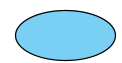
\includegraphics[width=0.1\linewidth]{images/ovalo.png}
    \end{minipage}
    \item Representa al actor que va a interactuar con el sistema.
    \begin{minipage}{0.2\textwidth}
        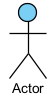
\includegraphics[width=0.1\linewidth]{images/actor.png}
    \end{minipage}
    \item Relación \texttt{<<extends>>}. Indica que un caso de uso puede ejecutarse a partir de otro.
    \item Relación \texttt{<<include>>}. Indica que un caso de uso debe ejecutarse a partir de otro.
\end{itemize}

La conexión entre un actor y un caso de uso se realiza mediante una línea como se muestra en la Figura 1.1.

\begin{figure}[htbp]
    \centering
    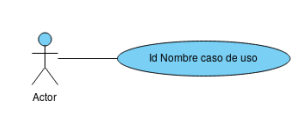
\includegraphics[width=0.4\textwidth]{images/interaccion.png}
    \caption{Interacción del actor con el caso de uso}
    \label{fig:interaccion-actor-caso-uso}
\end{figure}

Los casos de uso se encontrarán dentro de paquetes (representados por carpetas) indicando así que pertenecen a un mismo módulo, como se muestra en la Figura 1.2.

\begin{figure}[htbp]
    \centering
    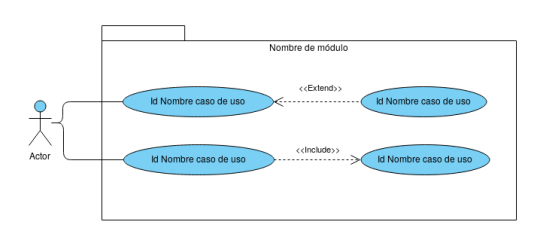
\includegraphics[width=0.6\textwidth]{images/interaccion2.png}
    \caption{Un Actor con varios casos de uso dentro de un módulo}
    \label{fig:actor-varios-casos-uso-modulo}
\end{figure}


%---------------------------------------------------------
\subsection{ Modelado Dinámico.}

Se centra en capturar y representar el comportamiento y las interacciones del sistema a lo largo del tiempo. Se utiliza para describir cómo los diferentes componentes del sistema interactúan entre sí y cómo se llevan a cabo las acciones y procesos. El modelado dinámico se realiza mediante diagramas de secuencia, diagramas de actividad, diagramas de estado y otras técnicas que permiten visualizar y analizar el flujo de eventos y el comportamiento dinámico del sistema.




%---------------------------------------------------------
\subsection{Modelos de Manejo de la Información}
Los modelos de manejo de la información se refieren a la representación y estructuración de los datos que serán almacenados y manipulados por el sistema. Estos modelos describen las entidades, atributos y relaciones entre los datos, y pueden incluir diagramas de entidad-relación, diagramas de clase y otros diagramas que ayudan a visualizar y comprender la estructura de los datos. El diseño de los modelos de manejo de la información busca garantizar la integridad, consistencia y eficiencia en la gestión de los datos, así como la adaptación a las necesidades específicas del sistema de la guardería.

Al abordar estos temas en el diseño del sistema de la guardería, se busca establecer una arquitectura sólida, modular y eficiente, así como una gestión efectiva de la información. Estos elementos son fundamentales para garantizar el rendimiento, la escalabilidad y la usabilidad del sistema, y para satisfacer las necesidades y expectativas de los usuarios finales.